\chapter{Domena terminologii}
\indent W ramach przygotowania projektu związanego z portfolio fotografa/filmowca, konieczne jest zapoznanie się z terminologią charakterystyczną dla tej domeny zainteresowania.
Wynikiem ekstensywnego badania domeny terminologii jest przedstawiony poniżej diagram. Zawiera on przykłady specjalistycznych terminów powiązanych z konkretnymi dziedzinami pracy
zawodowego fotografa bądź filmowca, przedstawiony w przystępny, zorganizowany sposób.
\begin{sidewaysfigure}
    \centering
    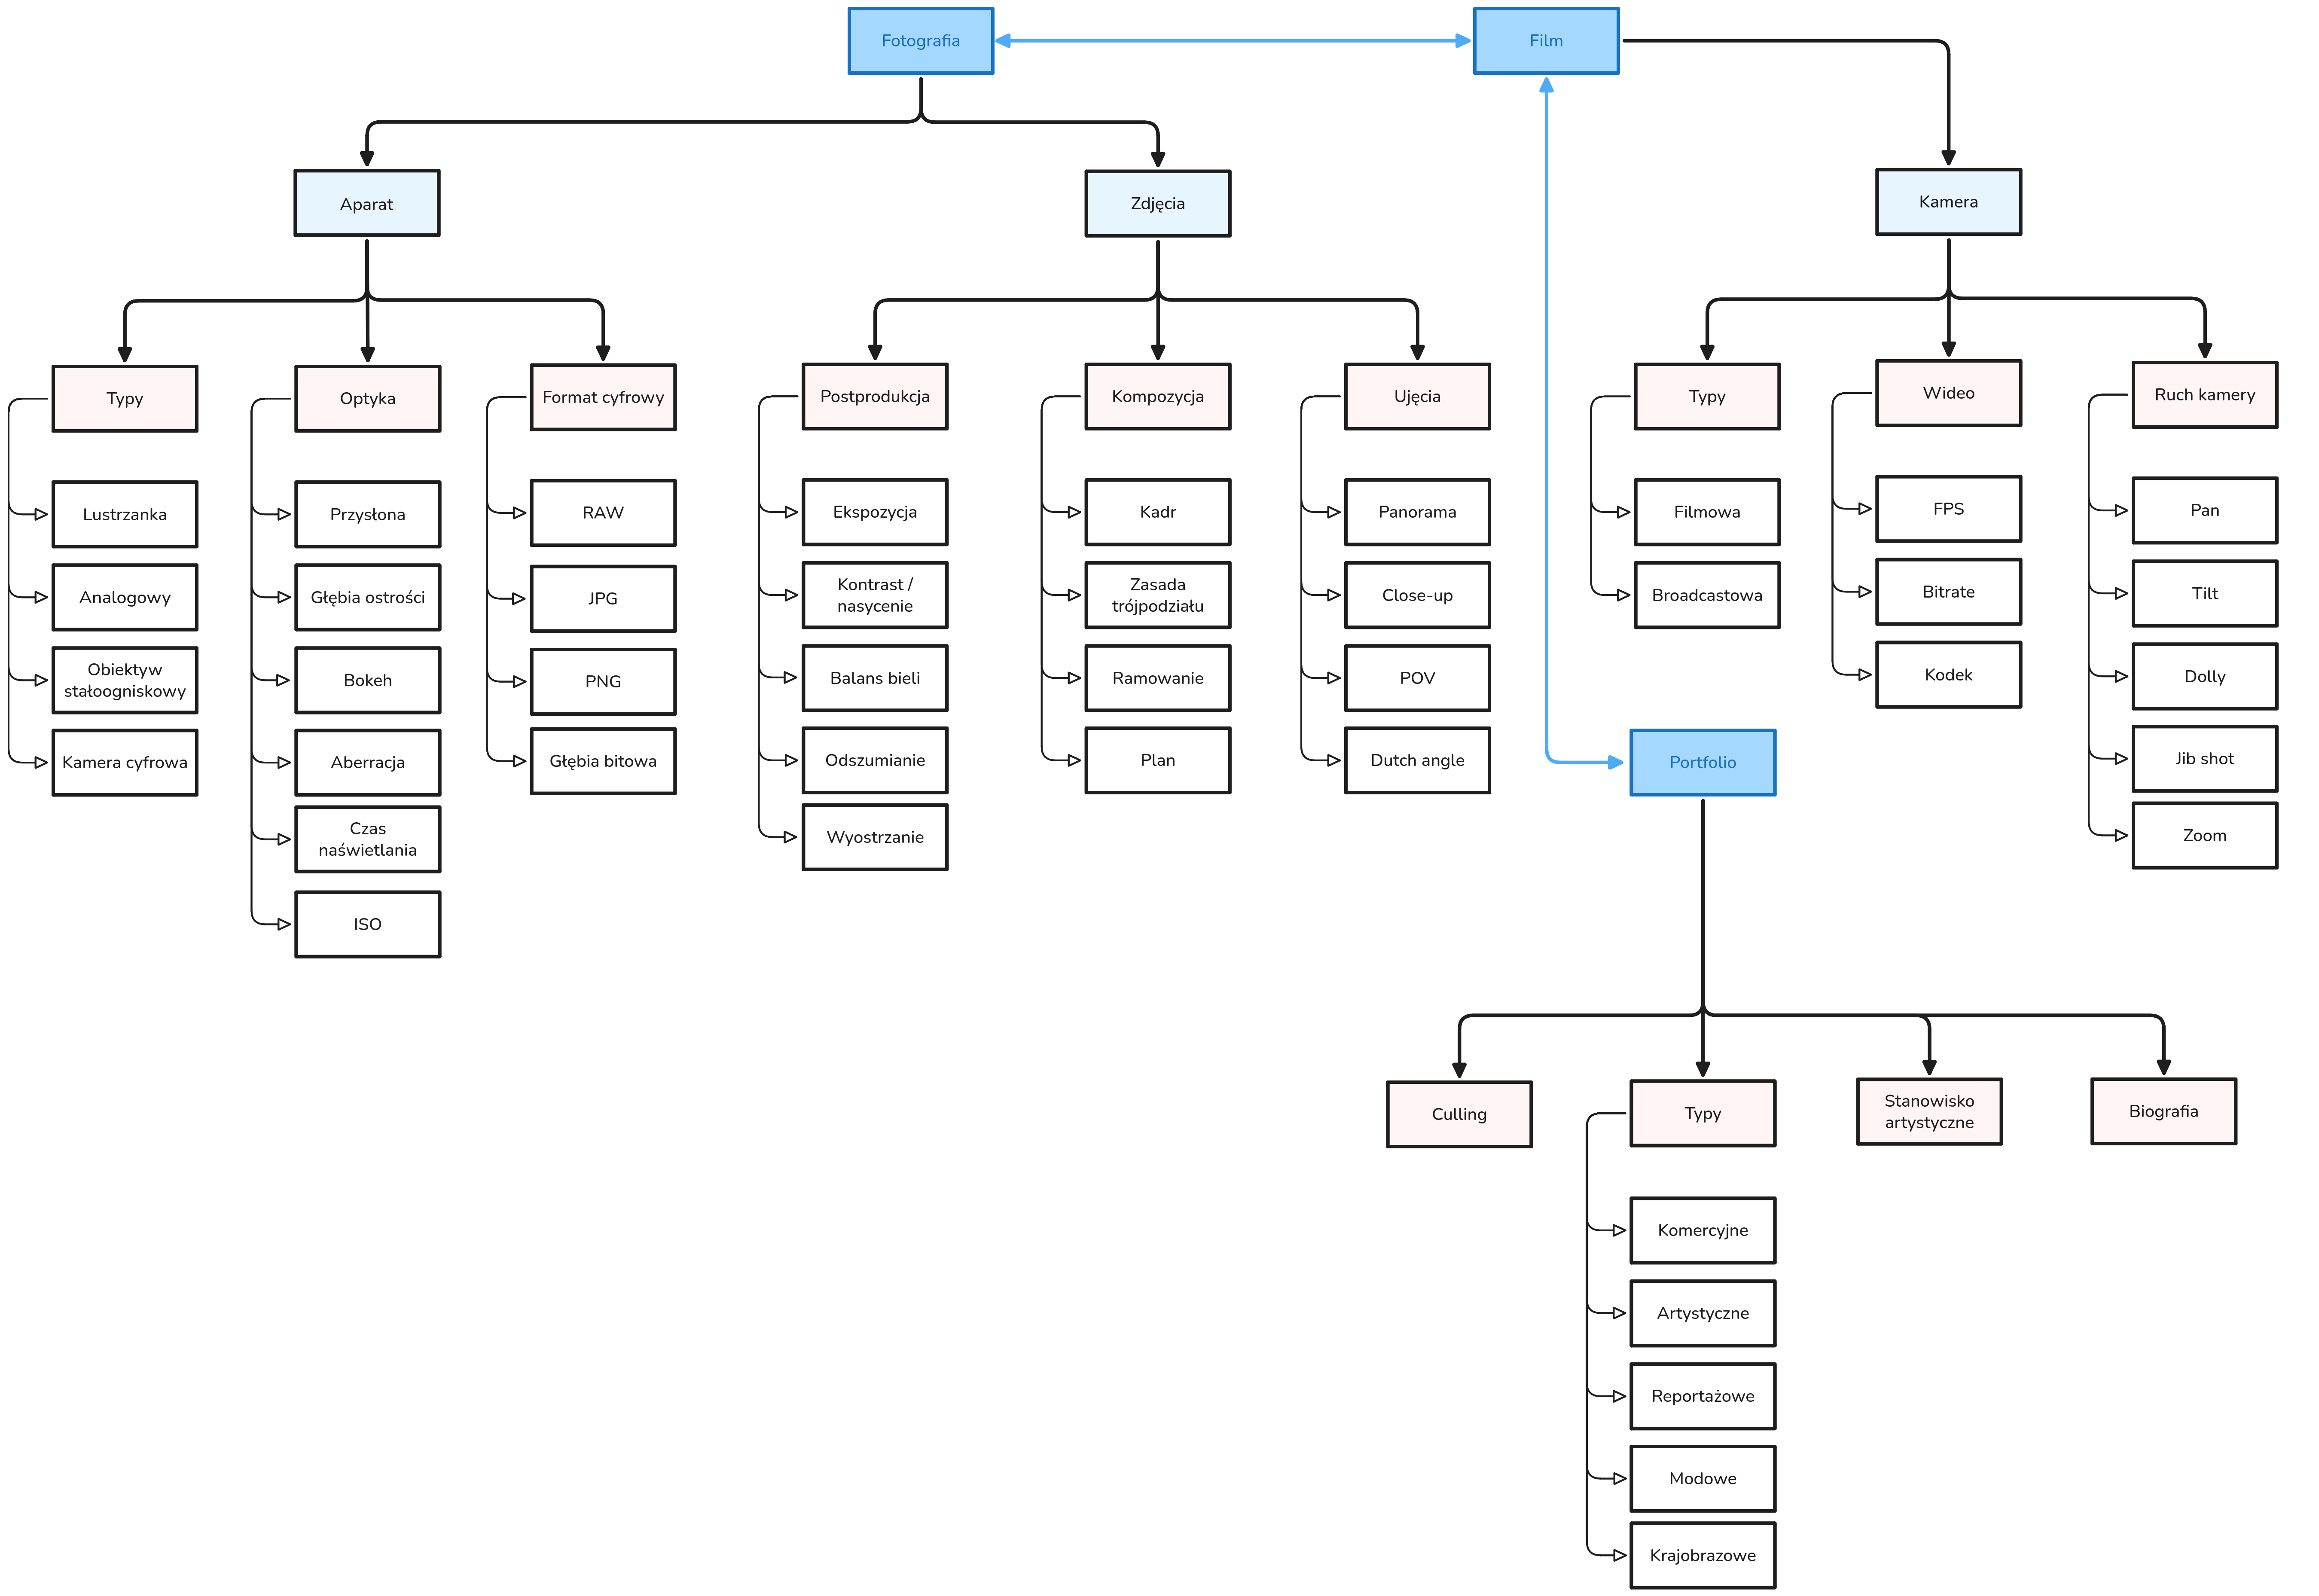
\includegraphics[scale=0.12]{../img/domena_terminologii.png}
\end{sidewaysfigure}

\chapter{Badanie preferencji klienta}
Witryna realizowana jest na życzenie Zleceniodawcy, wobec czego koniecznym stało się uzgodnienie ze Zleceniodawcą jego preferencji dotyczących sposobu
działania witryny, narzędzi jakie powinna oferować oraz preferencji dotyczących prezentacji witryny.

W tym celu przygotowano kwestionariusz mający nakreślić wymagania funkcjonalne oraz niefunkcjonalne, na podstawie udzielonych odpowiedzi.
Konieczne było dporecyzowanie oczekiwań dotyczących struktury strony, sposobu prezentacji portfolio, komunikacji z odbiorcą, identyfikacji wizualnej oraz wymagań związanych z dalszym zarządzaniem treścią. Na podstawie przeprowadzonej rozmowy możliwe było uszczegółowienie założeń projektowych oraz określenie zestawu funkcji, które powinny znaleźć się w finalnej wersji serwisu.

\section{Pytania}
\begin{enumerate}
    \item \textit{Jaki jest główny cel tej strony internetowej?}
    \item \textit{Kim są główni odbiorcy strony?}
    \item \textit{Jak użytkownik powinien doświadczać tej strony i jak powinien się po niej poruszać? Jakie podstrony lub sekcje powinny się na niej znaleźć, a co powinno pełnić rolę strony głównej?}
    \item \textit{Jakie obszary swojej działalności chce Pan pokazać na stronie?}
    \item \textit{W jaki sposób materiały wideo powinny być prezentowane, aby były wygodne i atrakcyjne w odbiorze?}
    \item \textit{Czy planuje Pan wykorzystywać na stronie filmy już opublikowane w innych serwisach, czy traktować tę stronę jako główne miejsce publikacji materiałów wideo?}
    \item \textit{W jaki sposób powinny być prezentowane zdjęcia?}
    \item \textit{Jakie formy kontaktu i nawiązania współpracy powinny znaleźć się na stronie?}
    \item \textit{Czy strona powinna działać tylko w jednym języku, czy w wielu? Jeśli w wielu, to w jakich?}
    \item \textit{Jaki charakter wizualny i styl strony najlepiej odpowiada Pana marce osobistej?}
    \item \textit{Czy po wdrożeniu będzie Pan chciał samodzielnie aktualizować treści na stronie?}
    \item \textit{Czy są jeszcze jakieś dodatkowe oczekiwania dotyczące działania strony, na przykład korzystania z niej na różnych urządzeniach, szybkości działania albo łatwości odnalezienia jej w sieci?}
\end{enumerate}

\section{Odpowiedź}
Na podstawie odpowiedzi zleceniodawcy ustalono, że serwis ma mieć charakter nowoczesnego portfolio, którego głównym zadaniem będzie prezentacja twórczości oraz pozyskiwanie nowych klientów. Strona główna powinna pełnić funkcję reprezentacyjną i już po wejściu prezentować charakter pracy twórcy, najważniejsze realizacje oraz wyraźne elementy zachęcające do kontaktu. Zleceniodawca wskazał również, że użytkownik powinien mieć możliwość intuicyjnego przechodzenia pomiędzy najważniejszymi obszarami serwisu. W strukturze strony powinny znaleźć się co najmniej: strona główna, sekcja lub podstrona poświęcona materiałom wideo, dedykowana strona przeznaczona dla fotografii, a także treści dotyczące autora, oferty i kontaktu.

Z przeprowadzonego wywiadu wynika, że na stronie mają zostać zaprezentowane dwa główne obszary działalności, czyli film oraz fotografia. Portfolio filmowe powinno być przedstawione w formie siatki umożliwiającej wygodne przeglądanie większej liczby materiałów, przy czym część realizacji może być celowo wyróżniona poprzez większy rozmiar elementu w układzie. Jednocześnie materiały powinny być uporządkowane tematycznie, tak aby użytkownik mógł łatwo odnaleźć interesujący go typ realizacji. W odpowiedziach zleceniodawcy wskazano także, że na stronie mają być prezentowane zarówno dłuższe formy filmowe, jak i krótsze materiały, takie jak rolki lub shorty. Ustalono również, że serwis nie ma być jedynym miejscem publikacji materiałów wideo, lecz powinien wykorzystywać filmy umieszczone już w zewnętrznych serwisach, takich jak YouTube czy Vimeo. W odniesieniu do fotografii zleceniodawca zaznaczył potrzebę przygotowania osobnej przestrzeni przeznaczonej dla zdjęć, umożliwiającej wygodne przeglądanie materiałów i ich powiększanie.

Zleceniodawca podkreślił, że strona ma nie tylko prezentować portfolio, ale również ułatwiać nawiązanie współpracy. Z tego względu w serwisie powinny znaleźć się czytelne formy kontaktu, w szczególności odnośniki do mediów społecznościowych, adres e-mail oraz funkcja umożliwiająca umawianie rozmów z klientem za pomocą kalendarza. Ważnym wymaganiem jest także wielojęzyczność serwisu. Strona powinna obsługiwać język polski oraz angielski, a preferowanym rozwiązaniem jest automatyczne wykrywanie języka użytkownika z możliwością ręcznej zmiany wersji językowej.

Istotnym elementem ustaleń była również warstwa wizualna projektu. Zleceniodawca oczekuje strony minimalistycznej, nowoczesnej i spójnej z jego marką osobistą. Serwis powinien wyróżniać się nie tylko estetyką, ale także odpowiednio dobranymi animacjami, które podkreślą charakter prezentowanej twórczości. Ponadto zleceniodawca zadeklarował chęć samodzielnego zarządzania zawartością strony po wdrożeniu, zwłaszcza w zakresie dodawania nowych materiałów i aktualizacji opisów. W odpowiedziach zaznaczono również, że strona powinna działać poprawnie zarówno na urządzeniach mobilnych, jak i desktopowych, ładować się sprawnie mimo obecności materiałów wizualnych oraz być przygotowana w sposób sprzyjający jej widoczności w wyszukiwarkach internetowych.

\chapter{Badanie preferencji użytkowników}
Zweryfikowano preferencje dotyczące potencjalnych użytkowników przygotowywanej witryny. Dokonano tego, przedstawiając pięciu wybranym uczestnikom kwestionariusz zawierający pytania dotyczące niuansów związanych z korzystaniem z portfolio fotografa.
Każdy z uczestników wybierał w skali od 1 do 5, gdzie 1 oznacza Nieważne/Niepotrzebne, natomiast 5 oznacza Bardzo ważne/Bardzo potrzebne.
\section{Pytania}
\begin{enumerate}
    \item \textit{Jak ważne jest dla Ciebie szybkie ładowanie strony?}
    \item \textit{Jak ważna jest możliwość szybkiego kontaktu (formularz/kalendarz) z twórcą?}
    \item \textit{Jak ważna jest dla Ciebie możliwość kontaktu przez preferowaną formę (formularz, email, telefon, social)?}
    \item \textit{Jak ważna jest możliwość obejrzenia materiałów video bezpośrednio na stronie?}
    \item \textit{Jak ważna jest estetyka i spójność wizualna (design) serwisu?}
    \item \textit{Jak ważne są dobre opisy projektów i meta-informacje (rola, rok, sprzęt)?}
    \item \textit{Czy ważne jest dla Ciebie filtrowanie treści (kategorie: komercyjne, teledyski, itp.)?}
    \item \textit{Jak ważna jest dla Ciebie responsywność i dobre działanie na urządzeniach mobilnych?}
    \item \textit{Jak ważne są dla Ciebie czytelne informacje o cenach/pakietach?}
    \item \textit{Jak ważne są dla Ciebie szczegółowe case studies (opis procesu, wyzwania, rozwiązania)?}
    \item \textit{Jak ważne są rekomendacje / referencje od klientów?}
    \item \textit{Jak ważne są dla Ciebie aktywne linki do mediów społecznościowych i regularne aktualizacje?}
    \item \textit{Jak ważna jest możliwość pobrania showreela lub materiałów?}
    \item \textit{Jak ważna jest dla Ciebie dostępność strony (WCAG, napisy do video itp.)?}
    \item \textit{Jak ważne jest dla Ciebie pokazanie materiałów zza kulis / behind-the-scenes?}
\end{enumerate}

\section{Odpowiedzi}

\bgroup
\def\arraystretch{1.2}
\begin{longtable}{| p{.03\textwidth} | p{.03\textwidth} | p{.03\textwidth} | p{.03\textwidth} | p{.03\textwidth} | p{.03\textwidth} | p{.03\textwidth} | p{.58\textwidth} |} 
\hline
\multicolumn{1}{|c|}{\multirow{2}{*}{\rotatebox{90}{\textbf{Pytanie\hspace{0.15cm}}}}} & \multicolumn{5}{|c|}{\textbf{Uczestnicy}} & \multicolumn{1}{|c|}{\multirow{2}{*}{\rotatebox{90}{\textbf{Średnia\hspace{0.2cm}}}}} & \multicolumn{1}{|c|}{\multirow{2}{*}{\textbf{Wnioski}}} \\[0.6cm] \cline{2-6}
\multicolumn{1}{|c|}{} & \multicolumn{1}{|c|}{\textbf{1}} & \multicolumn{1}{|c|}{\textbf{2}} & \multicolumn{1}{|c|}{\textbf{3}} & \multicolumn{1}{|c|}{\textbf{4}} & \multicolumn{1}{|c|}{\textbf{5}} & \multicolumn{1}{|c|}{} & \multicolumn{1}{|c|}{}\\ \hline\hline
\multicolumn{1}{|c|}{\textbf{1}} & \multicolumn{1}{|c|}{5} & \multicolumn{1}{|c|}{5} & \multicolumn{1}{|c|}{4} & \multicolumn{1}{|c|}{5} & \multicolumn{1}{|c|}{4} & \multicolumn{1}{|c|}{4.6} & Wydajność jest krytyczna \\ \hline
\multicolumn{1}{|c|}{\textbf{2}} & \multicolumn{1}{|c|}{5} & \multicolumn{1}{|c|}{4} & \multicolumn{1}{|c|}{5} & \multicolumn{1}{|c|}{4} & \multicolumn{1}{|c|}{5} & \multicolumn{1}{|c|}{4.6} & Kontakt i umawianie terminów są kluczowe. \\ \hline
\multicolumn{1}{|c|}{\textbf{3}} & \multicolumn{1}{|c|}{5} & \multicolumn{1}{|c|}{4} & \multicolumn{1}{|c|}{4} & \multicolumn{1}{|c|}{3} & \multicolumn{1}{|c|}{4} & \multicolumn{1}{|c|}{4.2} & Ważne jest oferować kilka opcji kontaktu, formularz + e-mail powinny być dostępne. \\ \hline
\multicolumn{1}{|c|}{\textbf{4}} & \multicolumn{1}{|c|}{5} & \multicolumn{1}{|c|}{5} & \multicolumn{1}{|c|}{4} & \multicolumn{1}{|c|}{5} & \multicolumn{1}{|c|}{5} & \multicolumn{1}{|c|}{4.8} & Osadzone odtwarzanie video jest bardzo istotne. \\ \hline
\multicolumn{1}{|c|}{\textbf{5}} & \multicolumn{1}{|c|}{5} & \multicolumn{1}{|c|}{4} & \multicolumn{1}{|c|}{5} & \multicolumn{1}{|c|}{4} & \multicolumn{1}{|c|}{5} & \multicolumn{1}{|c|}{4.6} & Design ma duże znaczenie dla odbioru portfolio. \\ \hline
\multicolumn{1}{|c|}{\textbf{6}} & \multicolumn{1}{|c|}{4} & \multicolumn{1}{|c|}{5} & \multicolumn{1}{|c|}{4} & \multicolumn{1}{|c|}{4} & \multicolumn{1}{|c|}{4} & \multicolumn{1}{|c|}{4.2} & Opisy pomagają klientom w decyzji, warto je uwzględnić. \\ \hline
\multicolumn{1}{|c|}{\textbf{7}} & \multicolumn{1}{|c|}{5} & \multicolumn{1}{|c|}{4} & \multicolumn{1}{|c|}{5} & \multicolumn{1}{|c|}{5} & \multicolumn{1}{|c|}{4} & \multicolumn{1}{|c|}{4.6} & Filtrowanie/kategoryzacja ułatwia nawigację. \\ \hline
\multicolumn{1}{|c|}{\textbf{8}} & \multicolumn{1}{|c|}{5} & \multicolumn{1}{|c|}{5} & \multicolumn{1}{|c|}{4} & \multicolumn{1}{|c|}{5} & \multicolumn{1}{|c|}{5} & \multicolumn{1}{|c|}{4.8} & Mobile-first i responsywność są krytyczne. \\ \hline
\multicolumn{1}{|c|}{\textbf{9}} & \multicolumn{1}{|c|}{4} & \multicolumn{1}{|c|}{3} & \multicolumn{1}{|c|}{4} & \multicolumn{1}{|c|}{4} & \multicolumn{1}{|c|}{3} & \multicolumn{1}{|c|}{3.6} & Część użytkowników oczekuje orientacyjnych cen. \\ \hline
\multicolumn{1}{|c|}{\textbf{10}} & \multicolumn{1}{|c|}{4} & \multicolumn{1}{|c|}{4} & \multicolumn{1}{|c|}{5} & \multicolumn{1}{|c|}{4} & \multicolumn{1}{|c|}{4} & \multicolumn{1}{|c|}{4.2} & Case studies zwiększają zaufanie i warto je pokazywać. \\ \hline
\multicolumn{1}{|c|}{\textbf{11}} & \multicolumn{1}{|c|}{4} & \multicolumn{1}{|c|}{5} & \multicolumn{1}{|c|}{4} & \multicolumn{1}{|c|}{3} & \multicolumn{1}{|c|}{4} & \multicolumn{1}{|c|}{4.0} & Referencje wspierają decyzję, powinny być widoczne. \\ \hline
\multicolumn{1}{|c|}{\textbf{12}} & \multicolumn{1}{|c|}{3} & \multicolumn{1}{|c|}{4} & \multicolumn{1}{|c|}{3} & \multicolumn{1}{|c|}{3} & \multicolumn{1}{|c|}{4} & \multicolumn{1}{|c|}{3.4} & Social media są przydatne, ale nie kluczowe dla wszystkich. \\ \hline
\multicolumn{1}{|c|}{\textbf{13}} & \multicolumn{1}{|c|}{2} & \multicolumn{1}{|c|}{3} & \multicolumn{1}{|c|}{2} & \multicolumn{1}{|c|}{2} & \multicolumn{1}{|c|}{3} & \multicolumn{1}{|c|}{2.2} & Pobieranie nie jest priorytetem dla większości użytkowników. \\ \hline
\multicolumn{1}{|c|}{\textbf{14}} & \multicolumn{1}{|c|}{3} & \multicolumn{1}{|c|}{3} & \multicolumn{1}{|c|}{2} & \multicolumn{1}{|c|}{3} & \multicolumn{1}{|c|}{4} & \multicolumn{1}{|c|}{3.0} & Dostępność ma znaczenie i warto zapewnić podstawowe wsparcie. \\ \hline
\multicolumn{1}{|c|}{\textbf{15}} & \multicolumn{1}{|c|}{2} & \multicolumn{1}{|c|}{3} & \multicolumn{1}{|c|}{3} & \multicolumn{1}{|c|}{2} & \multicolumn{1}{|c|}{3} & \multicolumn{1}{|c|}{2.6} & Materiały BTS są ciekawe, lecz nie kluczowe. \\ \hline
\end{longtable}
\egroup

\chapter{Wymagania projektu}

Na podstawie uzyskanych odpowiedzi określono następujący zestaw funkcji oraz wymagań dla projektowanego serwisu:

\bgroup
\def\arraystretch{1.2}
\begin{longtable}{| p{.40\textwidth} | p{.60\textwidth} |} 
\hline
\multicolumn{1}{|c|}{\textbf{Element serwisu / wymaganie}} & \multicolumn{1}{|c|}{\textbf{Uzasadnienie wynikające z wywiadu}} \\ \hline\hline
\textit{Landing page / strona główna prezentująca twórcę i charakter jego pracy        } & Zleceniodawca wskazał, że już po wejściu użytkownik powinien zobaczyć styl pracy autora, najważniejsze realizacje oraz otrzymać czytelne przejście do kontaktu. \\ \hline
\textit{Wyraźne CTA zachęcające do kontaktu                                            } & Głównym celem strony ma być nie tylko prezentacja portfolio, ale również pozyskiwanie klientów i inicjowanie współpracy.                                        \\ \hline
\textit{Czytelna struktura informacji i nawigacja                                      } & Zleceniodawca oczekuje intuicyjnego poruszania się użytkownika po stronie oraz jasnego podziału treści na główne obszary serwisu.                               \\ \hline
\textit{Podstrona lub sekcja poświęcona filmom                                         } & Jednym z dwóch podstawowych obszarów działalności wskazanych przez zleceniodawcę jest film, który wymaga odrębnej przestrzeni prezentacyjnej.                   \\ \hline
\textit{Dedykowana strona przeznaczona dla fotografii                                  } & Zleceniodawca zaznaczył, że fotografia powinna być prezentowana jako odrębny obszar portfolio, a nie jedynie jako dodatek do treści filmowych.                  \\ \hline
\textit{Siatka wideo w układzie typu masonry                                           } & W odpowiedziach wskazano potrzebę wygodnego przeglądania większej liczby materiałów filmowych w atrakcyjnej formie wizualnej.                                   \\ \hline
\textit{Możliwość wyróżniania wybranych filmów większym rozmiarem w siatce             } & Zleceniodawca oczekuje, że niektóre realizacje będą mogły zostać zaakcentowane wizualnie mocniej niż pozostałe.                                                 \\ \hline
\textit{Podział materiałów filmowych na kategorie                                      } & Użytkownik powinien mieć możliwość szybkiego odnalezienia interesującego go rodzaju realizacji, dlatego materiały muszą być uporządkowane tematycznie.          \\ \hline
\textit{Osobna prezentacja krótszych form, takich jak rolki / shorty                   } & Zleceniodawca wskazał, że obok klasycznych realizacji na stronie mają być obecne również krótsze materiały wideo.                                               \\ \hline
\textit{Integracja z zewnętrznymi serwisami wideo, np. YouTube i Vimeo                 } & Z wywiadu wynika, że filmy są już publikowane w innych serwisach i strona ma z nich korzystać, zamiast pełnić rolę jedynego repozytorium materiałów.            \\ \hline
\textit{Odtwarzanie materiałów bezpośrednio na stronie przez osadzenia                 } & Skoro materiały mają pochodzić z zewnętrznych platform, konieczne jest ich wygodne prezentowanie bez opuszczania strony.                                        \\ \hline
\textit{Galeria zdjęć z możliwością powiększania                                       } & Zleceniodawca oczekuje wygodnego przeglądania fotografii oraz możliwości oglądania ich w większym formacie.                                                     \\ \hline
\textit{Lightbox lub karuzela zdjęć                                                    } & Wynika to bezpośrednio z potrzeby płynnego przechodzenia między fotografiami i powiększania ich w obrębie strony.                                               \\ \hline
\textit{Sekcje „O mnie”, oferta i kontakt                                              } & Zleceniodawca wskazał, że poza samym portfolio użytkownik powinien mieć dostęp do informacji o autorze, zakresie usług oraz sposobie współpracy.                \\ \hline
\textit{Linki do mediów społecznościowych                                              } & Zleceniodawca oczekuje, że kontakt ze strony będzie możliwy także przez kanały, z których już korzysta.                                                         \\ \hline
\textit{Udostępnienie adresu e-mail                                                    } & E-mail został wskazany jako jedna z podstawowych i naturalnych form kontaktu.                                                                                   \\ \hline
\textit{Kalendarz do umawiania rozmów z klientem                                       } & Najważniejszą formą inicjowania współpracy ma być możliwość bezpośredniego umówienia rozmowy lub konsultacji przez stronę.                                      \\ \hline
\textit{Wsparcie wielu języków                                                         } & Zleceniodawca oczekuje, że strona będzie dostępna dla odbiorców posługujących się więcej niż jednym językiem.                                                   \\ \hline
\textit{Obsługa języka polskiego i angielskiego                                        } & W wywiadzie wskazano te dwie wersje językowe jako podstawowe.                                                                                                   \\ \hline
\textit{Automatyczne wykrywanie języka użytkownika z możliwością ręcznego przełączenia } & Taki sposób działania najlepiej odpowiada oczekiwaniu wygodnego dostępu do właściwej wersji językowej.                                                          \\ \hline
\textit{Dopracowana, spójna warstwa wizualna                                           } & Zleceniodawca podkreślił potrzebę zgodności strony z jego marką osobistą oraz wyróżniającego charakteru serwisu.                                                \\ \hline
\textit{Estetyka minimalistyczna i nowoczesna                                          } & Tak został określony preferowany kierunek stylistyczny projektu.                                                                                                \\ \hline
\textit{Zastosowanie animacji wzmacniających odbiór strony                             } & Zleceniodawca oczekuje, że serwis będzie wyróżniał się ruchem i detalami wizualnymi podkreślającymi charakter twórczości.                                       \\ \hline
\textit{Edycja treści przez headless CMS                                               } & Zleceniodawca chce samodzielnie dodawać nowe materiały i aktualizować treści bez konieczności ingerencji w kod.                                                 \\ \hline
\textit{Responsywność na urządzeniach mobilnych i desktopowych                         } & W wywiadzie wskazano, że użytkownicy będą korzystali ze strony z różnych typów urządzeń.                                                                        \\ \hline
\textit{Wysoka wydajność strony                                                        } & Mimo obecności licznych materiałów wizualnych serwis powinien działać płynnie i ładować się sprawnie.                                                           \\ \hline
\textit{Optymalizacja zasobów, zwłaszcza zdjęć i materiałów osadzanych                 } & Jest to konsekwencja oczekiwania dobrej wydajności przy jednoczesnym intensywnym wykorzystaniu mediów.                                                          \\ \hline
\textit{Przygotowanie strony z myślą o SEO                                             } & Zleceniodawca oczekuje, że serwis będzie łatwy do odnalezienia w sieci, co wymaga uwzględnienia zasad optymalizacji dla wyszukiwarek.                           \\ \hline


\end{longtable}
\egroup

\chapter{Architektura informacji}

Kluczowym z punktu widzenia tworzenia strony jest zadbanie o klarowne przekazanie informacji korzystającemu z witryny użytkownikowi.
Projektowana strona przyjmie sprawdzoną strukturę, ze stroną główną umożliwiającą łatwą nawigację do specjalistycznych części witryny.
Landing pełni rolę centralnego punktu nawigacyjnego, kierując użytkownika do kluczowych sekcji: portfolio (wideo i zdjęcia), strony „O mnie” oraz oferty. Najważniejszym elementem jest portfolio, które prowadzi do stron projektów, gdzie użytkownik otrzymuje szczegółowe informacje i zachętę do działania (CTA). 
Całość kończy się w sekcji kontakt/kalendarz, stanowiącej punkt finalny ścieżki. Każdy z elementów ścieżki pod portfolio jest osiągalny ze strony głównej. 
Równolegle działa panel CMS, który zasila wszystkie sekcje treścią i umożliwia ich aktualizację, pozostając poza bezpośrednią ścieżką użytkownika.

\begin{figure}[H]
    \centering
    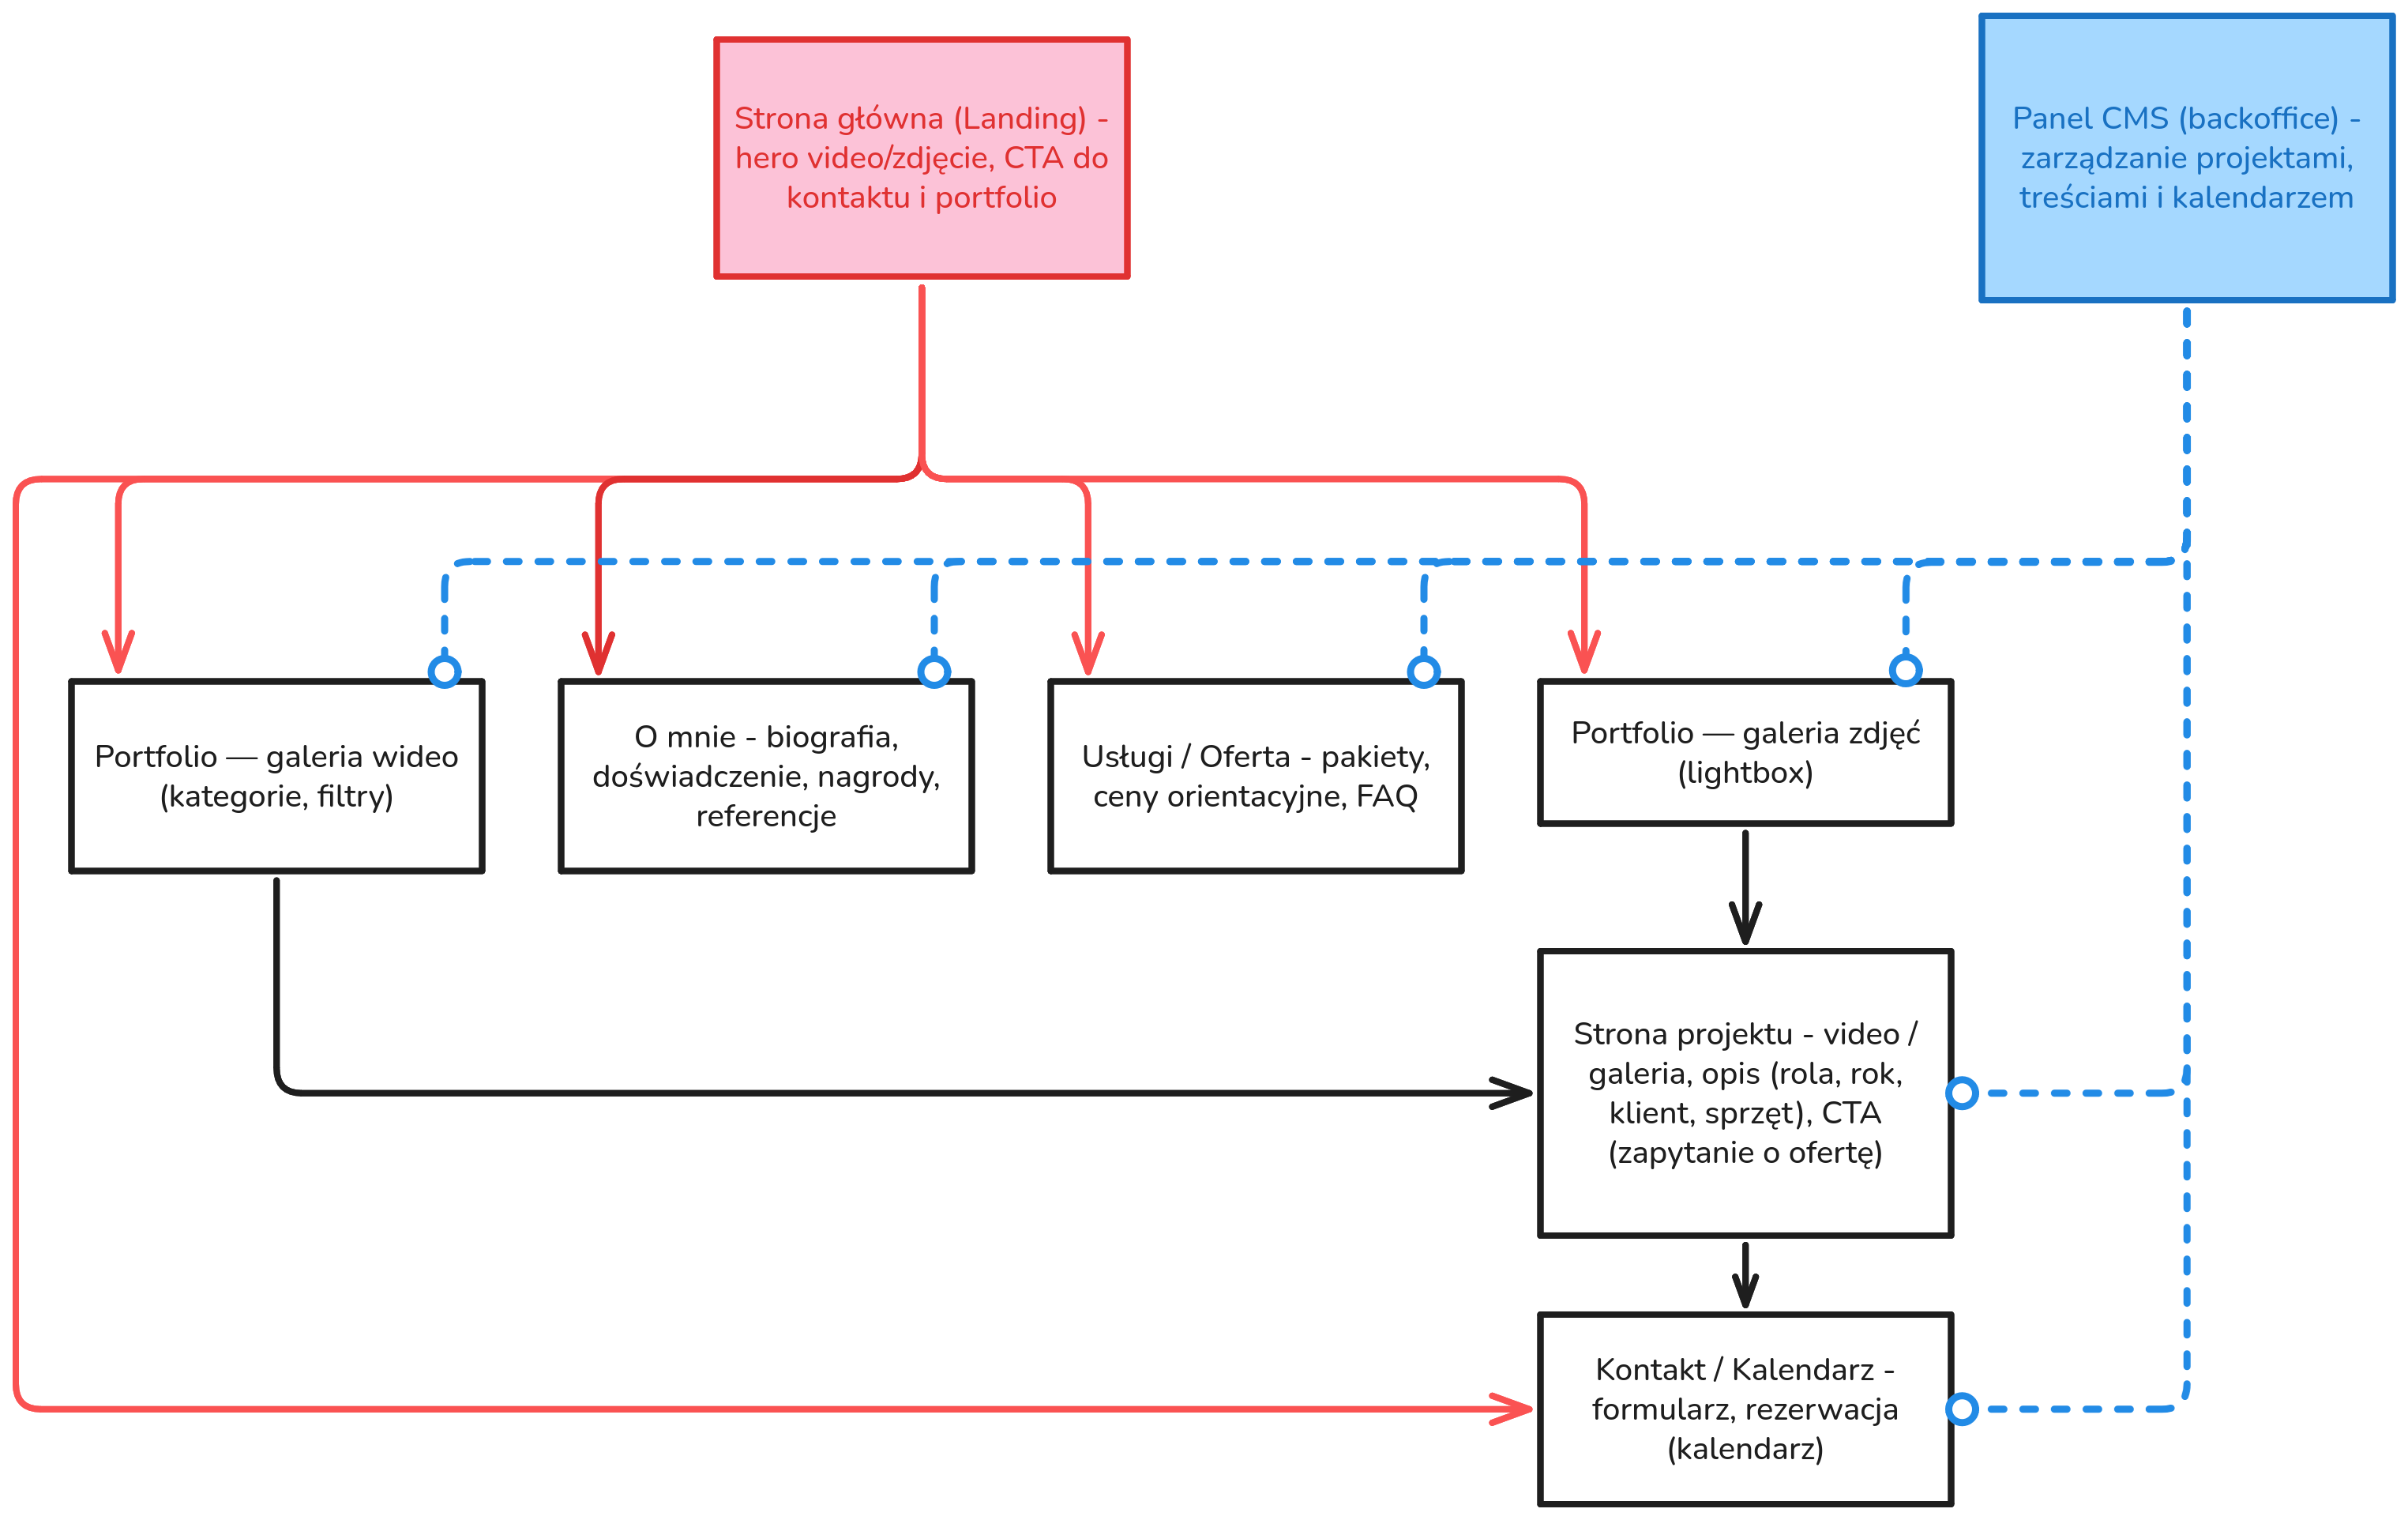
\includegraphics[scale=0.15]{../img/schemat_funkcjonalny.png}
\end{figure}

\chapter{Specyfikacja techniczna}
\section{Design}
Zgodnie z wypracowanymi wcześniej wymaganiami, proponuje się wstępne założenia dotyczące wyglądu witryny:

\subsection{Projekty okien}
\begin{itemize}
    \item Landing: układ hero (video/obraz), sekcja usług, ostatnie projekty, CTA.
    \item Portfolio grid: masonry z filtrami po kategorii i tagach.
    \item Strona projektu: player na górze, poniżej opis i galeria zdjęć.
    \item Kontakt: formularz + kalendarz + dane kontaktowe.
\end{itemize}

\subsection{Kolory i typografia}
\begin{itemize}
    \item Paleta kolorów:
    \begin{itemize}
        \item Primary: \#0F172A \hexcircle{0F172A}
        \item Accent: \#FF6B6B \hexcircle{FF6B6B}
        \item Secondary: \#F8FAFC \hexcircle{F8FAFC}
        \item Muted: \#94A3B8 \hexcircle{94A3B8}
    \end{itemize}
    \item Typografia:
    \begin{itemize}
        \item nagłówki — Inter / Montserrat
        \item tekst podstawowy — Roboto / system sans
    \end{itemize}
\end{itemize}

\section{Stos technologiczny}
Wstępnie proponuje się technologie umożliwiające realizację ww. wymagań:
\begin{itemize}
    \item Frontend: Next.js + React + TypeScript
    \item Stylowanie: Tailwind CSS
    \item CMS: Strapi (headless) lub alternatywy (Sanity, Contentful)
    \item Baza danych: PostgreSQL
    \item Hosting: Vercel (Next.js) + hosting CMS (zarządzany) lub self-host
\end{itemize}